\capitolo{Controllo del Moto per Trasmissione Rigida Senza Gioco}
Nell'industria i controllori sono di tipo P, PI, quindi le valutazioni saranno su questi.
Il modello di riferimento è quello classico del sistema motore, riduttore, carico a cui si aggiunge l'espressione base del motore:
\[
    C_m(t) = J \AccAng(t) + f \VelAng(t) + C_e (t) \\
    C_m(t) = K_T i(t)
\]

Che trasformata in Laplace diventa:
\[
\begin{cases}
    C_m(s)=(Js^2+fs)\theta(s) + C_e (s) \\
    C_m(s)=K_T I(s)
\end{cases}
\]

In cui sono state raggruppate tutte le varie inerzie, coefficienti di attrito e coppie legate a forze esterne.
Il sistema è a 1gdl.

\paragrafo{Schema Multi-Anello:}
In un sistema motore, riduttore, carico ci sono solitamente diversi anelli di controllo. Partendo dall'interno verso l'esterno ci sono gli anelli di: (tensione)\footnote{Nominato, ma non viene esaminato.} corrente, velocità e posizione.

\sottoparagrafo{Anello di corrente:}
L'anello di corrente è indipendente dalla meccanica; dipende dall'elettrica, dall'elettronica e dal controllo. Ha anche bande passanti caratteristiche ad alta frequenza \([kHz]\).

\sottoparagrafo{Anello di posizione:}
L'anello di posizione dipende: anello di velocità; trasduttore di posizione; controllo di posizione. In applicazioni tipiche ha banda passante inferiore i \(50 Hz\). 

\paragrafo{Feedback vs Feedforward:}
Nella trattazione classica dei controlli si tende a valutare soprattutto il sistema con feedback (catena chiusa), però tende a limitare le prestazioni. Un approccio più flessibile utilizza un feedback ben sintonizzato e un feedforward (catena aperta) basato sulla conoscenza (approssimata) del sistema fisico e del modello, che si traduce in una stima (nota a priori) di corrente\footnote{Nel caso dell'anello di velocità.} richiesta per la movimentazione.

\sezione{Anello di Velocità}
\import{Immagini/}{modello_complessivo}

L'anello di velocità dipende da: anello di corrente; meccanica; trasduttori di velocità; controllore di velocità.
Tipicamente ha bande passanti sul centinaio di \([Hz]\).

\sottosezione{Modello Semplificato 1}
Lo schematico in figura è quello completo, tuttavia in prima analisi conviene fare delle approssimazioni:
\begin{itemize}
    \item Coppie esterne vengono trascurate (valido per sovrapposizione degli effetti)
    \item Non utilizzo feedforward
    \item Trasduttore ideale, la misura non ha ritardi o errori, è come se il blocco relativo fosse 1
    \item Anello di corrente ideale, la corrente erogata, è come se il blocco relativo fosse 1
\end{itemize}

\import{Immagini/}{modello_semplificato_1}

\sottosottosezione{Controllo proporzionale}
Considerando il modello semplificato e l'utilizzo di un controllo di tipo proporzionale, ottengo che la funzione di trasferimento del sistema a catena chiusa è 
\[W(s)=\frac{K_{pv}K_T}{K_{pv}K_T+f}\frac{1}{1+s\frac{J}{f+K_{pv}+K_T}}\]
dove \(\tau = \frac{J}{f+K_{pv}+K_T}\) è la costante di tempo\footnote{Nota bene: si può parlare di costanti di tempo solo per sistemi del primo ordine.}.

\paragrafo{Banda passante:}
In un sistema del primo ordine la banda passante è data da \(\omega_B=\frac{1}{\tau}\), tuttavia considerando trascurabile l'attrito risulta \(\omega_B\simeq \frac{K_{pv}K_T}{J}\). Quest'ultima relazione permette facilmente di sintonizzare il controllore invertendo \(K_{pv}=\frac{\omega_B J}{K_T}\).

\paragrafo{Errore a regime:}
Per un sistema del primo ordine il guadagno in continua/regime è dato da \(\frac{K_{pv}K_T}{K_{pv}K_T+f}<1\), che è necessariamente minore di 1, ossia l'errore a regime non è nullo. Questo è molto negativo. Non potendo impostare un guadagno proporzionale infinito, occorre necessariamente valutare un controllore di altro tipo che permetta di ottenere un errore a regime nullo, di modo da avere un guadagno in continua unitario.

\sottosottosezione{Controllo Proporzionale Integrale}
Un controllore PI è del tipo \(C_V(s)=K_{pv}\frac{1+sT_{iv}}{sT_{iv}}\), per cui il sistema a catena chiusa diventa 
\[W_v(s)=\frac{K_{pv}K_T(1+sT_{iv})}{s^2T_{iv}J + sT_{iv}(f+K_{pv}K_T)+K_{pv}K_T}\]
Come era voluto, il sistema così ottenuto ha guadagno in continua unitario.
Però aumenta il numero di poli, diventa di secondo ordine\footnote{Fare riferimento a quanto presente in appendice \ref{sistemi_ordine_2}} (cosa che deve mettere in allarme per una serie di implicazione) e viene aggiunto uno zero reale (che ha anch'esso forti implicazioni). Tuttavia il grado relativo rimane 1.

\paragrafo{Effetto dello zero reale:}
Per valutare bene l'effetto dello zero nel sistema a catena chiusa adotto una parametrizzazione:
\[\frac{1+\frac{s}{\alpha \xi \omega_n}}{\left(\frac{s}{\omega_n}\right)^2+\frac{2\xi}{\omega_n}s+1}\]
Utilizzare \(\alpha\) permette di valutare dove si trova lo zero rispetto i poli del sistema
\[
\begin{cases}
\alpha >> 1 \text{ \ zero in alta frequenza} \\
\alpha \simeq 1 \text{ \ zero vicino ai poli} \\
\alpha << 1 \text{ \ zero in bassa frequenza}
\end{cases}
\]
In particolare si nota come la presenza dello zero vada a incrementare la sovraelongazione.

\textbf{La sovraelongazione dipende da \(\xi\) e dalla posizione dello zero.}

\begin{figure}[h]
    \centering
    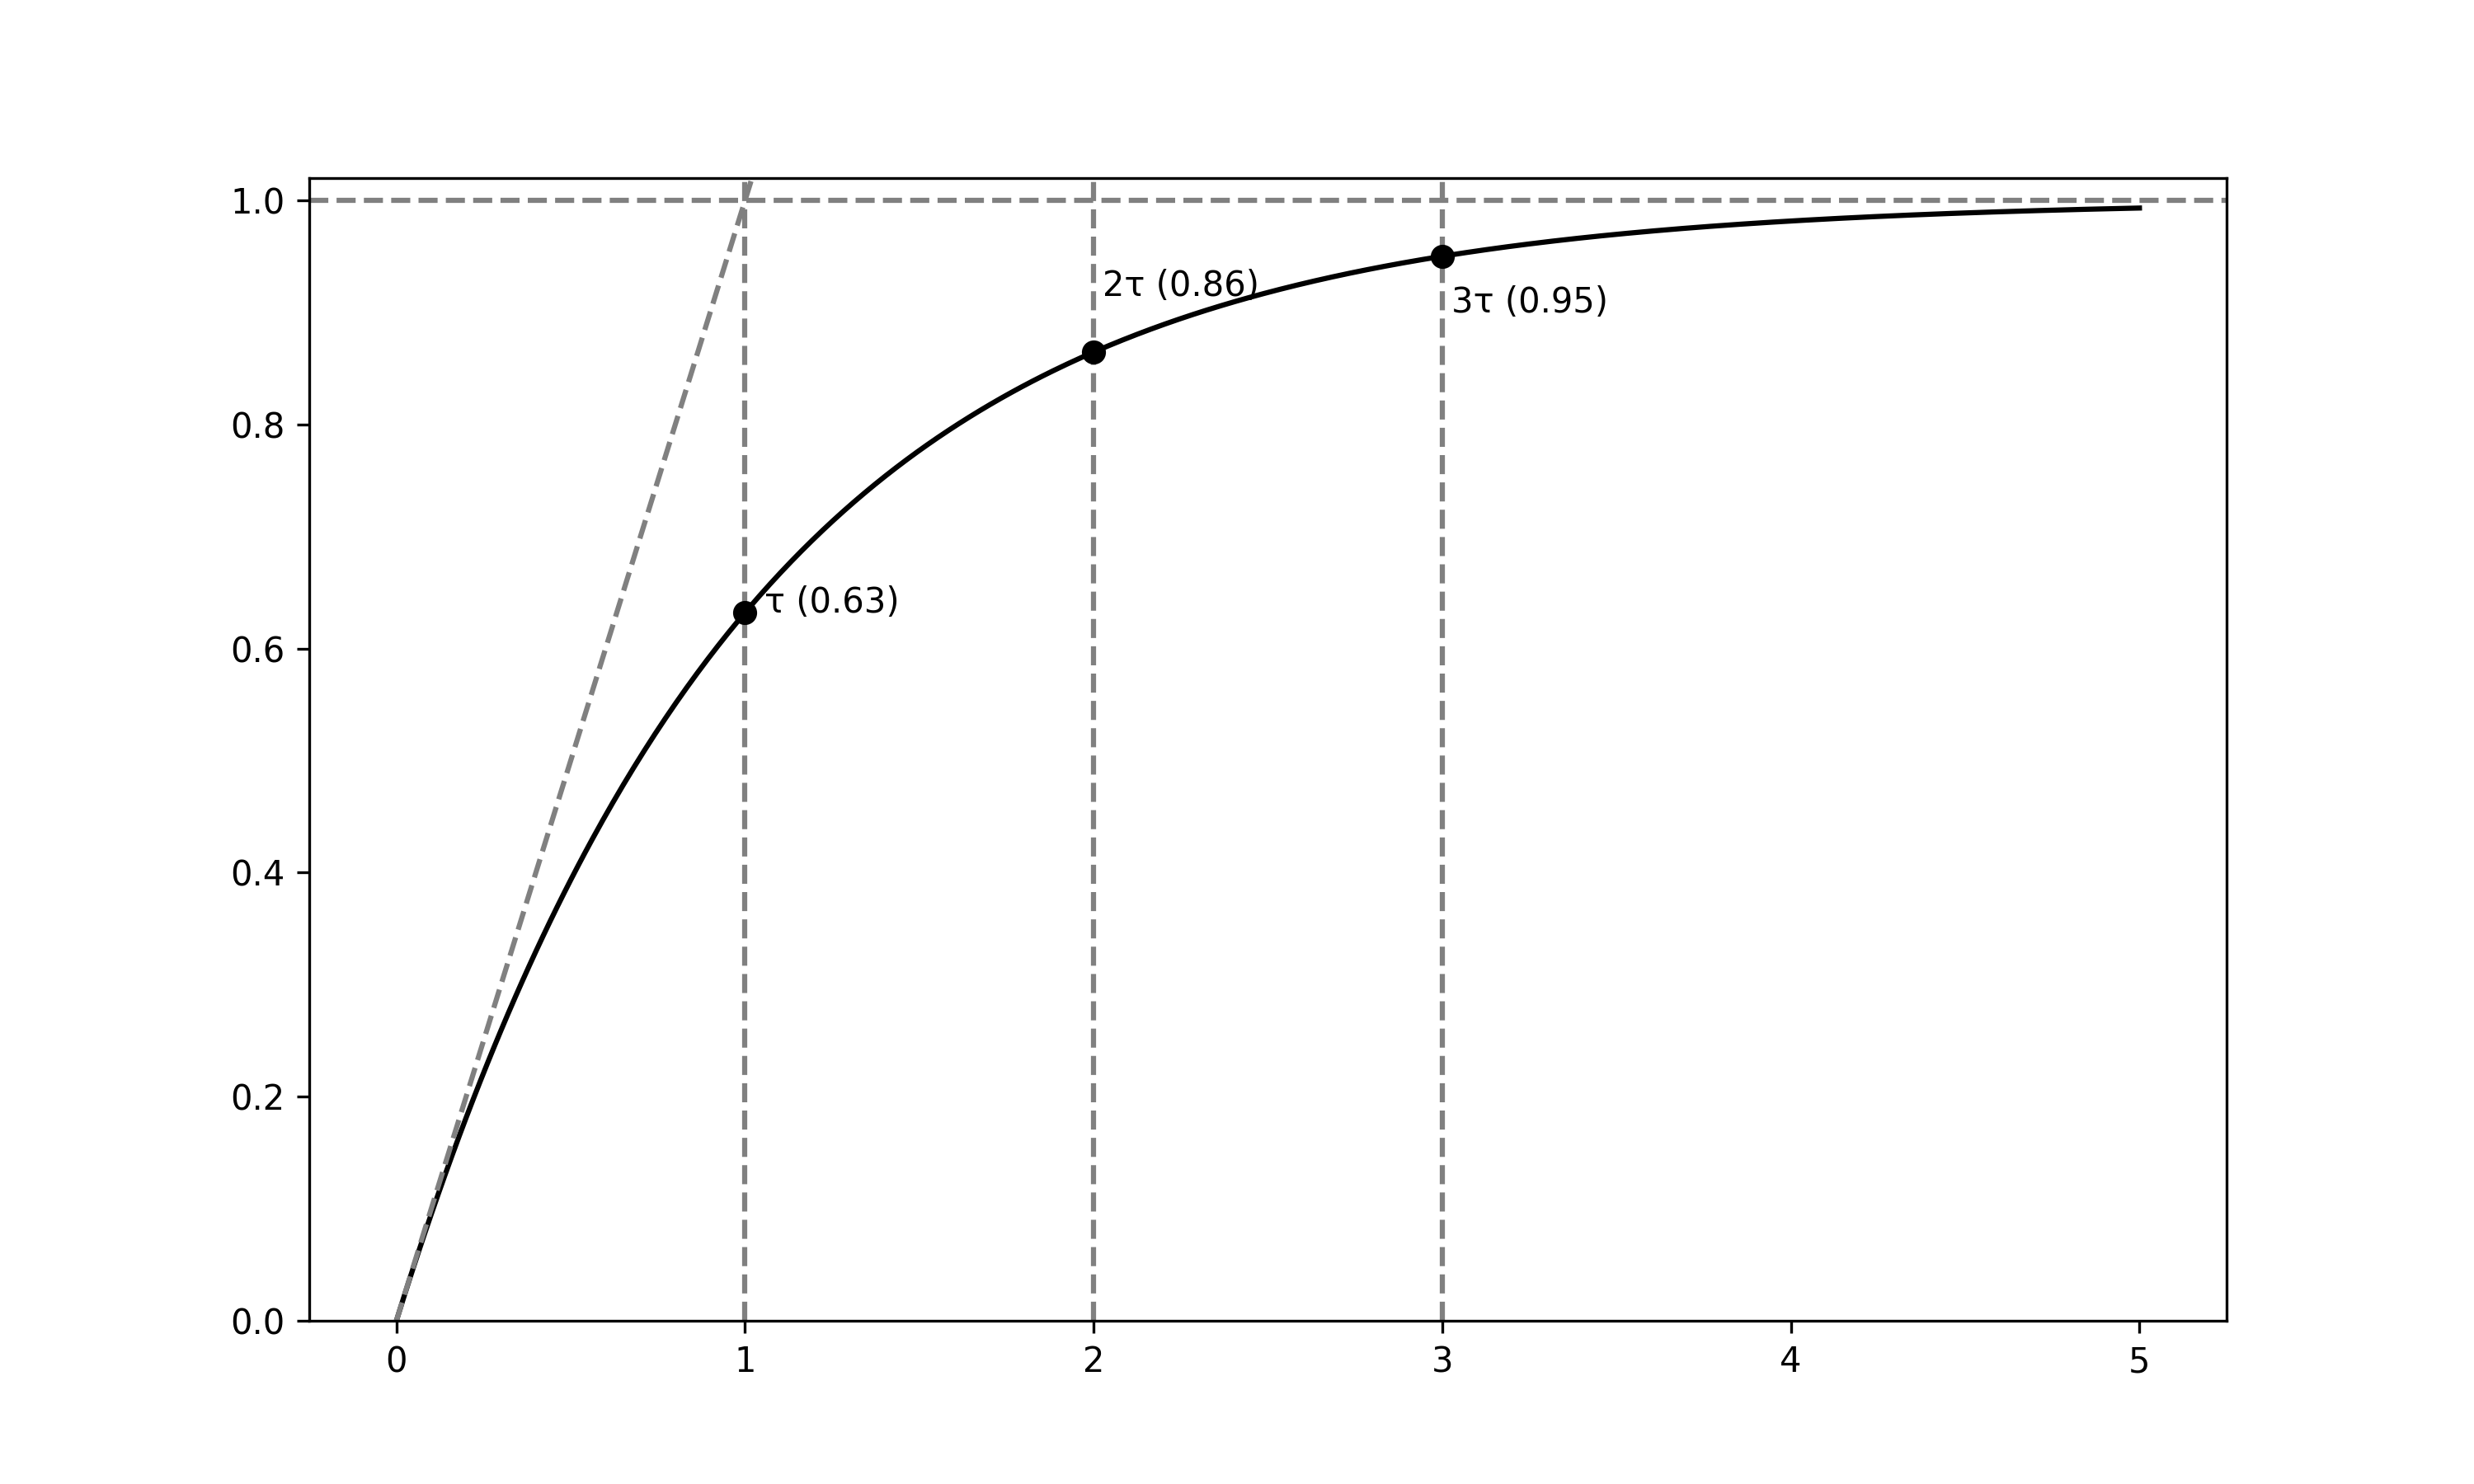
\includegraphics[width=0.45\textwidth]{Immagini/risposta_gradino_ord1_tempo.png}
    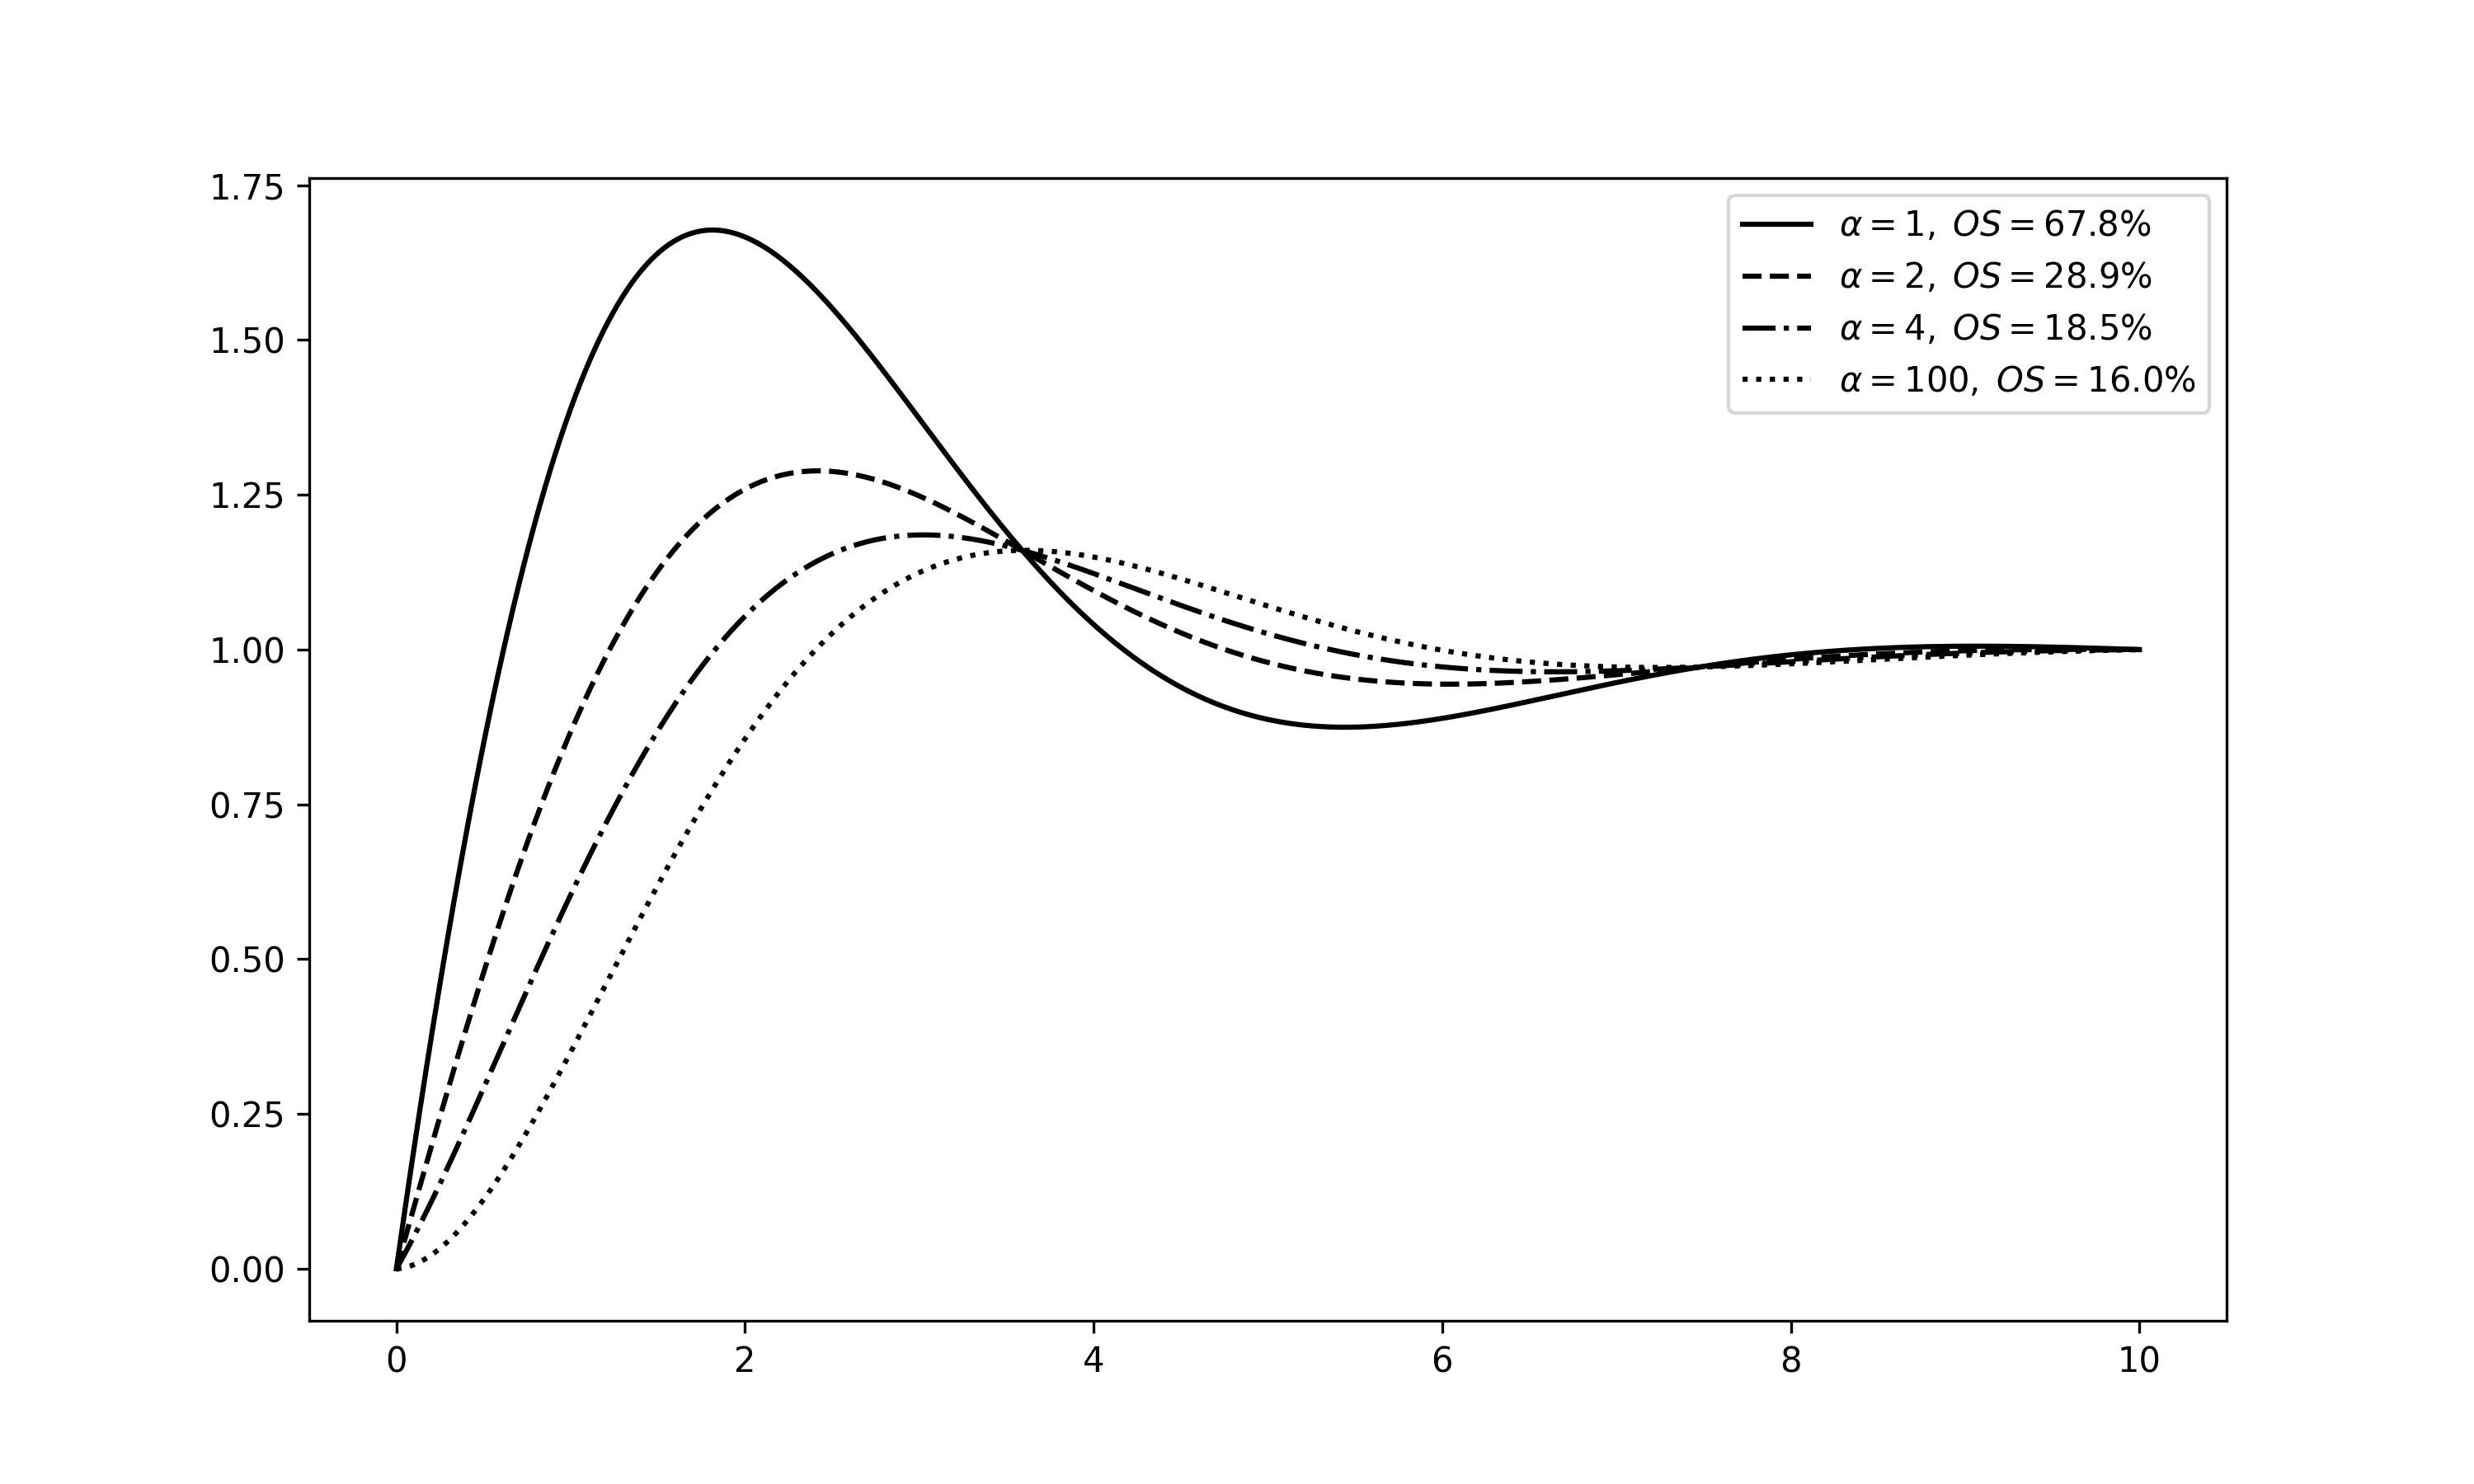
\includegraphics[width=0.45\textwidth]{Immagini/influenza_zero_su_sovraelong.png}
    \caption{Risposta al gradino di sistema di ordine 1 (sx); \(M_p(\alpha)\) in risposta al gradino (dx)}
\end{figure}

\sottoparagrafo{Scomposizione sovraelongazione poli e zero:}
A partire dal sistema a catena chiusa, vado a scomporre la componente legata al sistema del secondo ordine dal resto, cioè un sistema del secondo ordine derivato \(H(s)=\frac{1}{\left(\frac{s}{\omega_n}\right)^2+\frac{2\xi}{\omega_n}s+1} + \frac{1}{\alpha \xi \omega_n}\frac{s}{\left(\frac{s}{\omega_n}\right)^2+\frac{2\xi}{\omega_n}s+1}\), che nel tempo diventa \(h(t)=h_{2 ord}(t) + \frac{1}{\alpha \xi \omega_n} \derivata{h_{2 ord}(t)}{t}\).

Nella risposta al gradino avrò una componente legata alla risposta al gradino del sistema del secondo ordine e una componente legata alla risposta all'impulso\footnote{Impulso che è la derivata del gradino.} del sistema del secondo ordine.
\begin{itemize}
    \item Se cala lo smorzamento, a parità del resto, la sovraelongazione aumenta per effetto dello zero: \(\downarrow \xi \ \uparrow M_p\)
    \item Se \(\alpha >>1\) l'effetto legato allo zero diventa trascurabile
    \item Se \(\alpha <<1\) l'effetto legato allo zero è tanto più severo tanto è minore lo smorzamento
\end{itemize}

Quindi per attenuare la sovraelongazione conviene:
\begin{itemize}
    \item Posizionare gli zeri ad alta frequenza \(>> \xi \omega_n\)
    \item Se \(\xi << 1\) aumenta la sensibilità allo zero quindi lo zero va portato ancora  a più alta frequenza
    \item Se non è possibile intervenire su \(\alpha, \xi\), occorre intervenire sulla legge di moto
\end{itemize}

\begin{figure}[h]
    \centering
    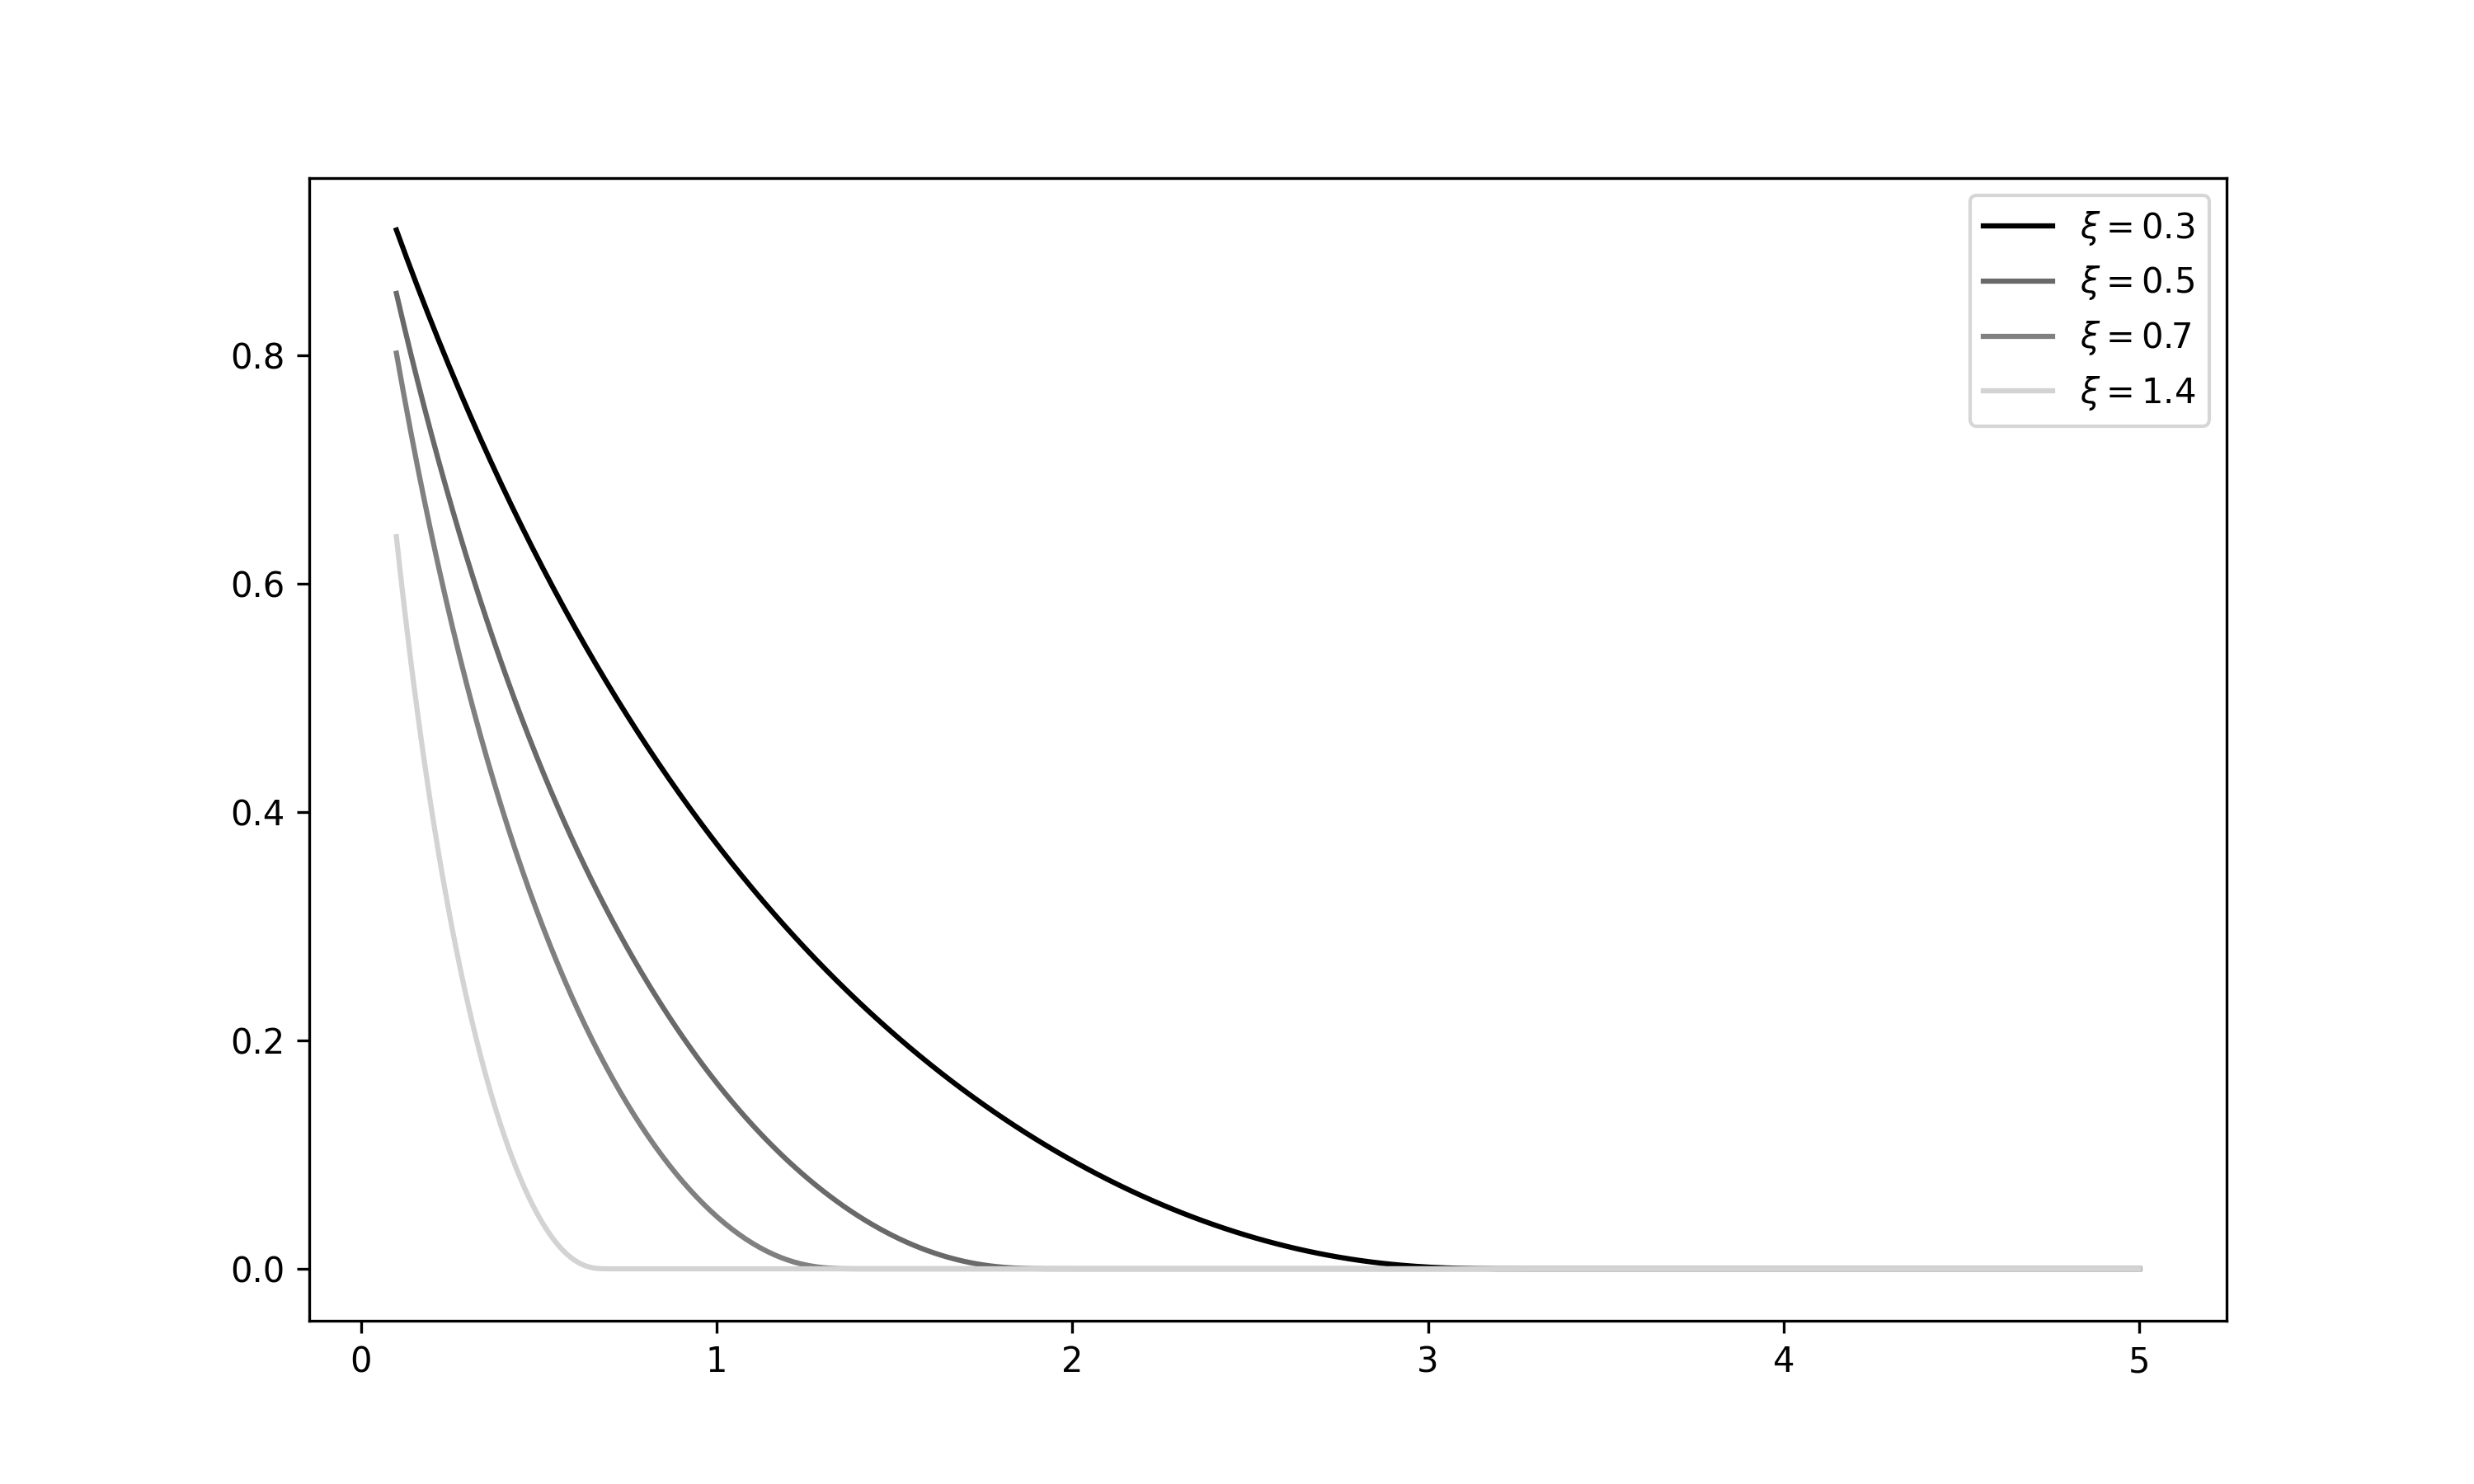
\includegraphics[width=0.6\textwidth]{Immagini/relazione_sovraelongazione.png}
    \caption{Relazione tra \(\alpha\) e \(M_p\)}
\end{figure}

\paragrafo{Banda passante:}
La banda passante di un sistema con controllore proporzionale è data da \(\omega_{bw}=\frac{K_{pv}K_T}{J}\).
Riscrivendo la funzione di trasferimento per il controllore PI come visto per sistemi massa molla smorzatore \(W(s)=\frac{K_{pv}K_T(1+sT_{iv})}{s^2M_{eq} + s C_{eq} + K_{eq}}\), si ottengono come poli del sistema \(S_{1,2}=\frac{-C_{eq}\pm\sqrt{C_{eq}^2-4M_{eq}K_{eq}}}{2M_{eq}}\). Il fattore di smorzamento vale \(\xi = \frac{C_{eq}}{2\sqrt{M_{eq}K_{eq}}}=\frac{\sqrt{T_{iv}}}{2}\sqrt{\frac{K_{pv}K_T}{J}}\), dove la banda passante del sistema valeva per controllore proporzionale \(\omega_{bw}=\frac{K_{pv}K_T}{J}\), quindi \(\xi=\frac{\sqrt{\omega_{bw}T_{iv}}}{2}\).
Lo zero del PI è in corrispondenza di \(\frac{1}{T_{iv}}\), invertendo l'espressione di \(\xi\), si può riscrivere \(\frac{1}{T_{iv}} = \frac{\omega_{bw}}{4\xi^2_{des}}\), ossia effettuando una opportuna scelta di fattore di smorzamento (\(\xi \in [0.7\div 1.4]\)  circa), la banda passante è ad un fattore 4 rispetto lo zero del PI, ossia la pulsazione di banda passante si ha quando l'effetto dell'integrale è già esaurito, quindi vale ancora la relazione della banda passante ricavata per controllore P:
\[\omega_{bw}=\frac{K_{pv}K_T}{J}\]

\paragrafo{Approccio tipico alla risoluzione:}
Dati limiti e specifiche sulla banda, si definisce una banda passante desiderata, si ricava il coefficiente proporzionale \(K_{pv}\), vanno aggiunte specifiche sullo smorzamento, quindi si ricava \(T_{iv}\).

\sottosottosezione{Legge di Moto}
A leggi di moto più dolci si associano sovraelongazioni legate allo zero più trascurabili. A leggi di moto non dolci si associano sovraelongazioni legate allo zero maggiori.

L'utilizzo della finestratura (tempo finito) e la discontinuità in accelerazione, portano ad avere infinite armoniche. 
Tutto ciò che viene attenuato dalla banda passante comporta distorsione della legge nel tempo, tendendo ad addolcire la legge, eliminando le discontinuità. Questo effetto è più rilevante per leggi non dolci. Tuttavia, in una RtR, perdere armoniche porta a non ottenere arresto all'istante finale.

\paragrafo{Esempi:}
In termini di leggi di moto la risposta al gradino è non dolce, perciò gli effetti delle sovraelongazioni sono particolarmente acuiti.

\begin{figure}[h]
    \centering
    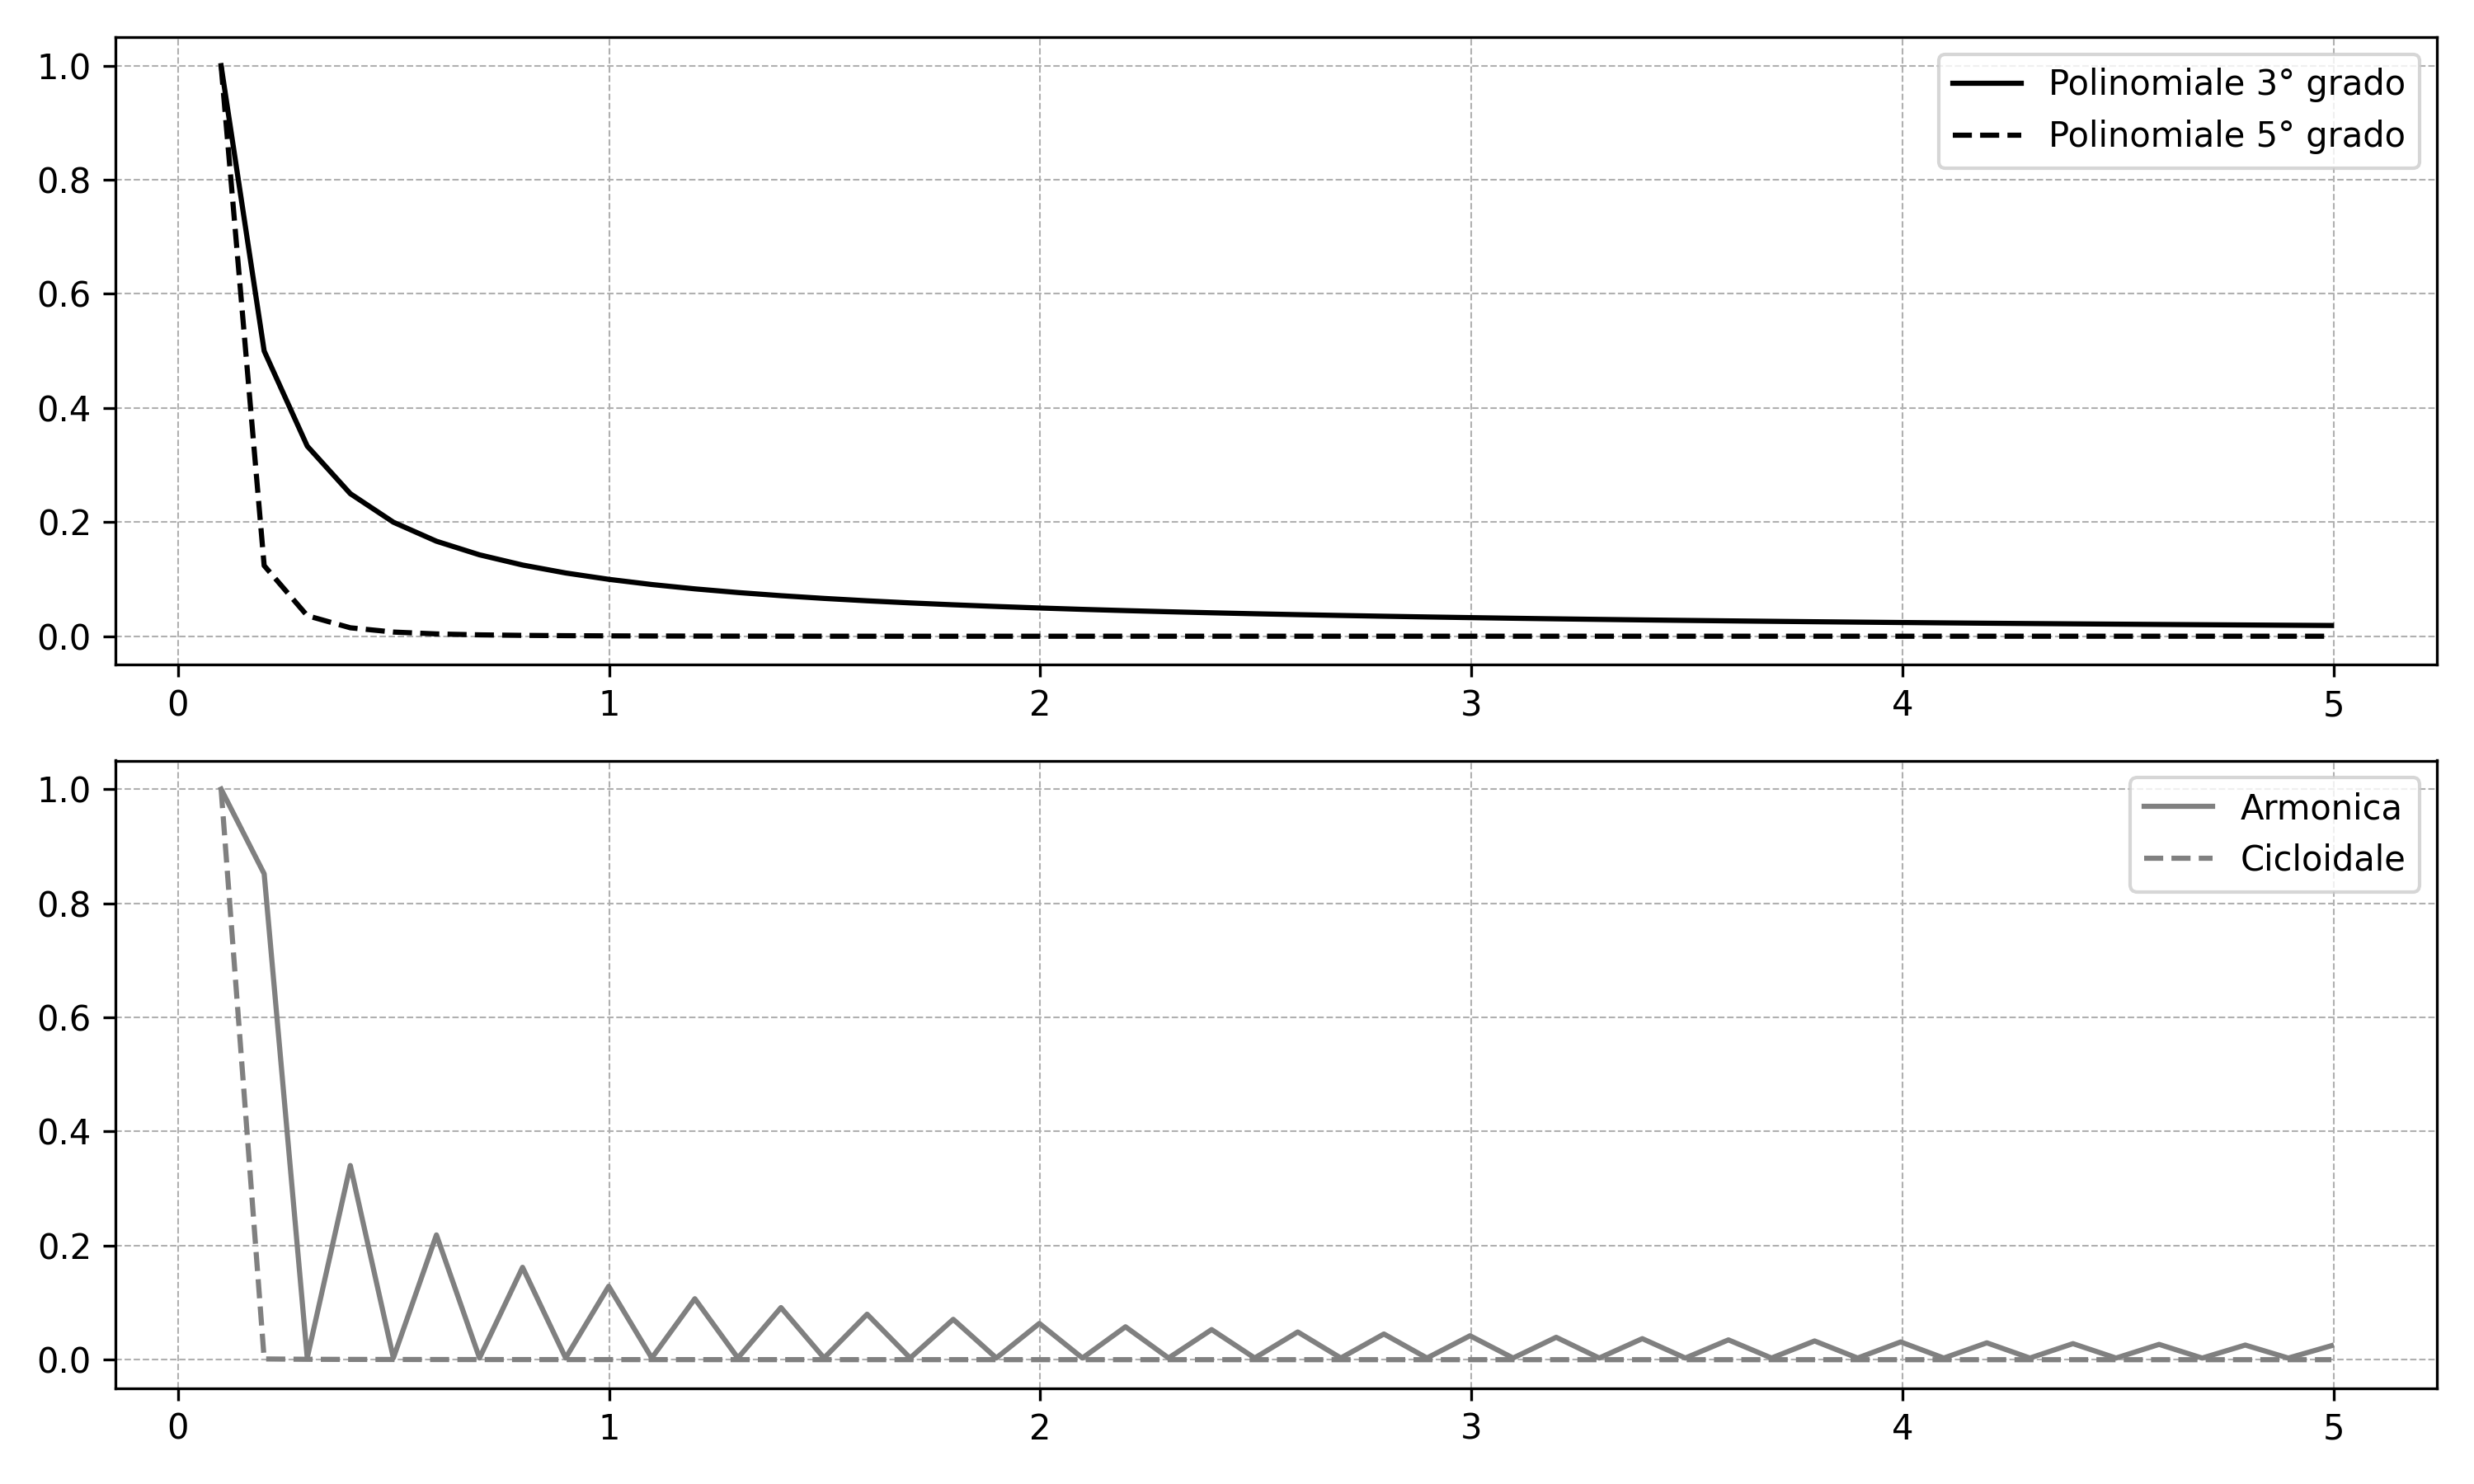
\includegraphics[width=0.6\textwidth]{Immagini/fft_leggi_di_moto.png}
    \caption{FFT delle principali leggi di moto}
\end{figure}

\paragrafo{Riduzione del tempo di moto:}
La riduzione del tempo di moto peggiora gli effetti di distorsione perché: le armoniche aumentano di frequenza, perciò è più facile vengano attenuate; inoltre le singole armoniche vedono un incremento in termini di ampiezza \(\propto \frac{1}{T^2}\).

\paragrafo{Limiti all'aumento della banda passante:}

\import{Immagini/}{modello_senza_feedforward}


% inserire in appendice criterio di stabilità di bode